% Relaxation dispersion.
%%%%%%%%%%%%%%%%%%%%%%%%

\chapter[Relaxation dispersion]{The analysis of relaxation dispersion} \label{ch: relax-disp}
\index{relaxation dispersion|textbf}

\begin{figure*}[h]
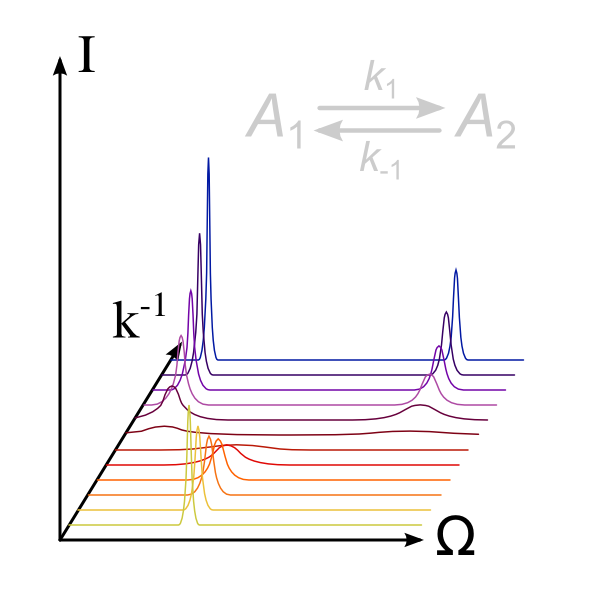
\includegraphics[width=5cm, bb=0 0 1701 1701]{graphics/analyses/relax_disp_600x600}
\end{figure*}


% Introduction.
%%%%%%%%%%%%%%%

\section{Introduction to relaxation dispersion}

Relaxation dispersion is the experimental modulation of chemical exchange relaxation.  For the $\Ronerho$-type experiment in which the nucleus of interest is spin-locked, either the spin-lock field strength or the offset between the spin-lock pulse and the chemical shift of the spins is used to modulate the exchange.  For the CPMG-type experiment, varying the time between the pulses modules the exchange.  Both experiment types are handled by relax.


% The models.
%~~~~~~~~~~~~

\subsection{The modelling of dispersion data}

For a system under the influence of chemical exchange, the evolution of the transverse magnetisation is given by the \citet{Bloch46} equations as modified by \citet{McConnell58} for chemical exchange -- the Bloch-McConnell equations.
For a two state exchange jumping between states A and B, the equation is:

\begin{equation} \label{eq: Bloch-McConnell}
    \frac{d}{dt} \left[ 
        \begin{array}{c}
            M_A^+(t) \\
            M_B^+(t)
        \end{array}
    \right] = \left[
        \begin{array}{cc}
            -i\Omega_A-\RtwozeroA-\pB\kex & \pA\kex \\
            \pB\kex & -i\Omega_B-\RtwozeroB-\pA\kex \\
        \end{array}
    \right] \left[
        \begin{array}{c}
            M_A^+(t) \\
            M_B^+(t)
        \end{array}
    \right] .
\end{equation}

The solution to this equation then Fourier transformed to produce the NMR spectrum.  However the analytic or closed-form frequency-domain solution remains intractable.

Solutions can nevertheless be found by either making assumptions or restrictions about the exchange process and then analytically solving~\ref{eq: Bloch-McConnell} or by finding numeric solutions.
The modelling of relaxation dispersion data can hence be catergorised into these two distinct methodologies:

\begin{description}
\item[Analytical models:]\index{relaxation dispersion!Analytical model}  Optimisation of models based on analytical, closed-form expressions derived from the Bloch-McConnell equations subject to certain conditions (see Section~\ref{sect: dispersion: analytic CPMG models} on page~\pageref{sect: dispersion: analytic CPMG models} and Section~\ref{sect: dispersion: analytic R1rho models} on page~\pageref{sect: dispersion: analytic R1rho models}).
\item[Numerical models:]\index{relaxation dispersion!Numerical model}  Optimisation of models based on numerically solving the Bloch-McConnell equations (see Section~\ref{sect: dispersion: numeric CPMG models} on page~\pageref{sect: dispersion: numeric CPMG models} and Section~\ref{sect: dispersion: numeric R1rho models} on page~\pageref{sect: dispersion: numeric R1rho models}).
\end{description}



% Implemented models.
%~~~~~~~~~~~~~~~~~~~~

\subsection{Implemented models}
\label{sect: dispersion: implemented models}

A number of analytic models are supported within relax.
If the model you are interested in is not available, see Section~\ref{sect: dispersion: model tutorial} on page~\pageref{sect: dispersion: model tutorial} for how new models can be added to relax.
The analytic models are dependant upon whether the data originates from a CPMG-type or $\Ronerho$-type experiment.
For the CPMG-type experiments, the models currently supported are:

\begin{description}
\item[`R2eff':]\index{relaxation dispersion!R2eff model}  This is the model used to determine the $\Rtwoeff$ values and errors required as the base data for all other models.  See Section~\ref{sect: dispersion: R2eff model} on page~\pageref{sect: dispersion: R2eff model}.
\item[`No Rex':]\index{relaxation dispersion!No Rex model}  This is the model for no chemical exchange being present.  See Section~\ref{sect: dispersion: No Rex model} on page~\pageref{sect: dispersion: No Rex model}.
\item[`LM63':]\index{relaxation dispersion!LM63 model}  The original \citet{LuzMeiboom63} 2-site fast exchange equation with parameters $\{\Rtwozero, \dots, \Phiex, \kex\}$.  See Section~\ref{sect: dispersion: LM63 model} on page~\pageref{sect: dispersion: LM63 model}.
\item[`LM63 3-site':]\index{relaxation dispersion!LM63 3-site model}  The original \citet{LuzMeiboom63} 3-site fast exchange equation with parameters $\{\Rtwozero, \dots, \PhiexB, \kB, \PhiexC, \kC\}$.  The equations of \citet{OConnell09} can be used to approximately convert the parameters $\{\PhiexB, \kB, \PhiexC, \kC\}$ to more biologically relevant parameters.  See Section~\ref{sect: dispersion: LM63 3-site model} on page~\pageref{sect: dispersion: LM63 3-site model}.
\item[`CR72':]\index{relaxation dispersion!CR72 model}  The reduced \citet{CarverRichards72} 2-site equation for all time scales whereby the simplification $\RtwozeroA = \RtwozeroB$ is assumed.  It has the parameters $\{\Rtwozero, \dots, \pA, \dw, \kex\}$.  See Section~\ref{sect: dispersion: CR72 model} on page~\pageref{sect: dispersion: CR72 model}.
\item[`CR72 full':]\index{relaxation dispersion!CR72 full model}  The full \citet{CarverRichards72} 2-site equation for all time scales with parameters $\{\RtwozeroA, \RtwozeroB, \dots, \pA, \dw, \kex\}$.  See Section~\ref{sect: dispersion: CR72 full model} on page~\pageref{sect: dispersion: CR72 full model}.
\item[`IT99':]\index{relaxation dispersion!IT99 model}  The \citet{IshimaTorchia99} 2-site model for all time scales with $\pA \gg \pB$ and with parameters $\{\Rtwozero, \dots, \Phiex, \pA.\dw^2, \kex\}$.  See Section~\ref{sect: dispersion: IT99 model} on page~\pageref{sect: dispersion: IT99 model}.
\item[`TSMFK01':]\index{relaxation dispersion!TSMFK01 model}  The \citet{Tollinger01}  2-site very-slow exchange model for time scales within range of microsecond to second time scale.
Applicable in the limit of slow exchange, when $|\RtwozeroA - \RtwozeroB| \ll \kAB, \kBA \ll 1/\taucpmg$.  $2*\taucpmg$ is the time between successive 180 degree pulses. Parameters are $\{\RtwozeroA, \dots, \dw, \kAB\}$.  See Section~\ref{sect: dispersion: TSMFK01 model} on page~\pageref{sect: dispersion: TSMFK01 model}.
\end{description}

For the $\Ronerho$-type experiment, the currently supported models are:

\begin{description}
\item[`R2eff':]\index{relaxation dispersion!R2eff model}  This is the same model model as for the CPMG-type experiments except that the $\Ronerho$ and not $\Rtwoeff$ values are determined.  See Section~\ref{sect: dispersion: R2eff model} on page~\pageref{sect: dispersion: R2eff model}.
\item[`No Rex':]\index{relaxation dispersion!No Rex model}  This is the model for no chemical exchange being present.  See Section~\ref{sect: dispersion: No Rex model} on page~\pageref{sect: dispersion: No Rex model}.
\item[`M61':]\index{relaxation dispersion!M61 model}  The \citet{Meiboom61} 2-site fast exchange equation for on-resonance data with parameters $\{\Ronerhoprime, \dots, \Phiex, \kex\}$.  See Section~\ref{sect: dispersion: M61 model} on page~\pageref{sect: dispersion: M61 model}.
\item[`DPL94':]\index{relaxation dispersion!DPL94 model}  The \citet{Davis94} 2-site fast exchange equation for off-resonance data with parameters $\{\Ronerhoprime, \dots, \Phiex, \kex\}$.  See Section~\ref{sect: dispersion: DPL94 model} on page~\pageref{sect: dispersion: DPL94 model}.
\item[`M61 skew':]\index{relaxation dispersion!M61 skew model}  The \citet{Meiboom61} 2-site equation for all time scales with $\pA \gg \pB$ and with parameters $\{\Ronerhoprime, \dots, \pA, \dw, \kex\}$.  This model is disabled by default in the dispersion auto-analysis.  See Section~\ref{sect: dispersion: M61 skew model} on page~\pageref{sect: dispersion: M61 skew model}.
\item[`TP02':]\index{relaxation dispersion!TP02 model}  The \citet{TrottPalmer02} 2-site equation for all time scales with parameters $\{\Ronerhoprime, \dots, \pA, \dw, \kex\}$.  See Section~\ref{sect: dispersion: TP02 model} on page~\pageref{sect: dispersion: TP02 model}.
\end{description}


Like the analytic models, a number of numerical models are supported within relax.
These models are also dependant upon whether the data originates from a CPMG-type or $\Ronerho$-type experiment.
For the CPMG-type experiments, the models currently supported are:

\begin{description}
\item[`R2eff':]\index{relaxation dispersion!R2eff model}  This is the model used to determine the $\Rtwoeff$ values and errors required as the base data for all other models.  See Section~\ref{sect: dispersion: R2eff model} on page~\pageref{sect: dispersion: R2eff model}.
\item[`No Rex':]\index{relaxation dispersion!No Rex model}  This is the model for no chemical exchange being present.  See Section~\ref{sect: dispersion: No Rex model} on page~\pageref{sect: dispersion: No Rex model}.
\item[`NS CPMG 2-site 3D':]\index{relaxation dispersion!NS CPMG 2-site 3D model}  The reduced model for 2-site exchange using 3D magnetisation vectors whereby the simplification $\RtwozeroA = \RtwozeroB$ is assumed.  It has the parameters $\{\Rtwozero, \dots, \pA, \dw, \kex\}$.  See Section~\ref{sect: dispersion: NS CPMG 2-site 3D model} on page~\pageref{sect: dispersion: NS CPMG 2-site 3D model}.
\item[`NS CPMG 2-site 3D full':]\index{relaxation dispersion!NS CPMG 2-site 3D full model}  The full model for 2-site exchange using 3D magnetisation vectors with parameters $\{\RtwozeroA, \RtwozeroB, \dots, \pA, \dw, \kex\}$.  See Section~\ref{sect: dispersion: NS CPMG 2-site 3D full model} on page~\pageref{sect: dispersion: NS CPMG 2-site 3D full model}.
\item[`NS CPMG 2-site star':]\index{relaxation dispersion!NS CPMG 2-site star model}  The reduced model for 2-site exchange using complex conjugate matrices whereby the simplification $\RtwozeroA = \RtwozeroB$ is assumed.  It has the parameters $\{\Rtwozero, \dots, \pA, \dw, \kex\}$.  See Section~\ref{sect: dispersion: NS CPMG 2-site star model} on page~\pageref{sect: dispersion: NS CPMG 2-site star model}.
\item[`NS CPMG 2-site star full':]\index{relaxation dispersion!NS CPMG 2-site star full model}  The full model for 2-site exchange using complex conjugate matrices with parameters $\{\RtwozeroA, \RtwozeroB, \dots, \pA, \dw, \kex\}$.  See Section~\ref{sect: dispersion: NS CPMG 2-site star full model} on page~\pageref{sect: dispersion: NS CPMG 2-site star full model}.
\item[`NS CPMG 2-site expanded':]\index{relaxation dispersion!NS CPMG 2-site expanded model}  A model for 2-site exchange expanded using Maple by Nikolai Skrynnikov.  It has the parameters $\{\Rtwozero, \dots, \pA, \dw, \kex\}$.  See Section~\ref{sect: dispersion: NS CPMG 2-site expanded model} on page~\pageref{sect: dispersion: NS CPMG 2-site expanded model}.
\end{description}


For the $\Ronerho$-type experiment, the models currently supported are:

\begin{description}
\item[`R2eff':]\index{relaxation dispersion!R2eff model}  This is the model used to determine the $\Rtwoeff$ values and errors required as the base data for all other models.  See Section~\ref{sect: dispersion: R2eff model} on page~\pageref{sect: dispersion: R2eff model}.
\item[`No Rex':]\index{relaxation dispersion!No Rex model}  This is the model for no chemical exchange being present.  See Section~\ref{sect: dispersion: No Rex model} on page~\pageref{sect: dispersion: No Rex model}.
\item[`NS R1rho 2-site':]\index{relaxation dispersion!NS R1rho 2-site model}  The model for 2-site exchange using 3D magnetisation vectors.  It has the parameters $\{\Ronerhoprime, \dots, \pA, \dw, \kex\}$.  See Section~\ref{sect: dispersion: NS R1rho 2-site model} on page~\pageref{sect: dispersion: NS R1rho 2-site model}.
\end{description}





% Dispersion model summary.
%~~~~~~~~~~~~~~~~~~~~~~~~~~

\subsection{Dispersion model summary}

Except for `R2eff' and `No Rex', all models can be fit to clusterings of spins, or spin blocks.
The models are described in more detail below and summarised in Table~\ref{table: CPMG dispersion models} for CPMG-type experiments and Table~\ref{table: R1rho dispersion models} for $\Ronerho$-type experiments.
The parameters are given in Table~\ref{table: dispersion parameters}.

\begin{sidewaystable}
\begin{center}
\caption{The parameters of relaxation dispersion.}
\begin{longtable}{llll}
\toprule
Parameter          & Equation                       & Description                                                                   & Units \\
\midrule
$\nucpmg$          & $1 / (2 \taucpmg)$             & CPMG frequency                                                                & Hz \\
$\taucpmg$         & $1 / (2 \nucpmg)$              & Delay between CPMG $\pi$ pulses                                               & s \\
$T_\textrm{relax}$ & -                              & The relaxation delay period                                                   & s \\
$I_0$              & -                              & Reference peak intensity when $T_\textrm{relax}$ is zero                      & - \\
$I_1$              & -                              & Peak intensity for a given $\nucpmg$ or spin-lock field strength $\omega_1$   & - \\
$\Rtwozero$        & -                              & $\Rtwo$ relaxation rate in the absence of exchange                            & rad.s$^{-1}$ \\
$\RtwozeroA$       & -                              & $\Rtwo$ relaxation rate for state A in the absence of exchange                & rad.s$^{-1}$ \\
$\RtwozeroB$       & -                              & $\Rtwo$ relaxation rate for state B in the absence of exchange                & rad.s$^{-1}$ \\
$\Ronerhoprime$    & -                              & $\Ronerho$ relaxation rate in the absence of exchange                         & rad.s$^{-1}$ \\
$\aveoffset$       & $\aveomega - \omegarf$         & The average resonance offset in the rotating frame                            & rad.s$^{-1}$ \\
$\omegaA$          & -                              & The Larmor frequency of the spin in state A                                   & rad.s$^{-1}$ \\
$\omegaB$          & -                              & The Larmor frequency of the spin in state B                                   & rad.s$^{-1}$ \\
$\aveomega$        & $\pA\omegaA + \pB\omegaB$      & The population averaged Larmor frequency of the spin                          & rad.s$^{-1}$ \\
$\omegaone$        & -                              & Spin-lock field strength, i.e. the amplitude of the rf field                  & rad.s$^{-1}$ \\
$\omegae$          & $\sqrt(\aveoffset^2 + \omegaone^2)$  & Effective field in the rotating frame                                   & rad.s$^{-1}$ \\
$\omegarf$         & -                              & Spin-lock offset, i.e. the frequency of the rf field                          & rad.s$^{-1}$ \\
$\theta$           & $\arctan \left( \frac{\omegaone}{\aveoffset} \right)$  & Rotating frame tilt angle                             & rad \\
$\kAB$             & $\pB\kex$                      & The forward exchange rate from state A to state B                             & rad.s$^{-1}$ \\
$\kBA$             & $\pA\kex$                      & The reverse exchange rate from state B to state A                             & rad.s$^{-1}$ \\
$\kex$             & $1 / (2 \tex)$                 & Chemical exchange rate constant                                               & rad.s$^{-1}$ \\
$\kexB$            & $\kAB + \kBA$                  & Chemical exchange rate constant between sites A and B                         & rad.s$^{-1}$ \\
$\kexC$            & $\kAC + \kCA$                  & Chemical exchange rate constant between sites A and C                         & rad.s$^{-1}$ \\
$\kB$              & $\approx \kexB$                & Approximate chemical exchange rate constant between sites A and B             & rad.s$^{-1}$ \\
$\kC$              & $\approx \kexC$                & Approximate chemical exchange rate constant between sites A and C             & rad.s$^{-1}$ \\
$\tex$             & $1 / (2 \kex)$                 & Time of exchange                                                              & s.rad$^{-1}$ \\
$\pA$              & -                              & Population of state A                                                         & - \\
$\pB$              & -                              & Population of state B                                                         & - \\
$\dw$              & -                              & Chemical shift difference between the two states                              & rad.s$^{-1}$ (stored as ppm) \\
$\Phiex$           & $\pA\pB\dw^2$                  & Fast exchange factor                                                          & rad$^2$.s$^{-2}$ (stored as ppm$^2$) \\
$\PhiexB$          & See \ref{eq: disp phiexB} on page \pageref{eq: disp phiexB} & Fast exchange factor between sites A and B       & rad$^2$.s$^{-2}$ (stored as ppm$^2$) \\
$\PhiexC$          & See \ref{eq: disp phiexC} on page \pageref{eq: disp phiexC} & Fast exchange factor between sites A and C       & rad$^2$.s$^{-2}$ (stored as ppm$^2$) \\
\bottomrule
\label{table: dispersion parameters}
\end{longtable}
\end{center}
\end{sidewaystable}



% The base models.
%%%%%%%%%%%%%%%%%%

\clearpage

\section{The base dispersion models}
\label{sect: dispersion: base models}
\index{relaxation dispersion!Base model|textbf}


% R2eff model.
%~~~~~~~~~~~~~

\subsection{The R2eff model}
\label{sect: dispersion: R2eff model}
\index{relaxation dispersion!R2eff model|textbf}

This is the simplest of all models in that the dispersion component of the base data -- the peak intensity values -- is not modelled.  It is used to determine either the $\Rtwoeff$ or $\Ronerho$ values and errors as required for the base data for all other models.  It can be selected by setting the model to `R2eff'.  Depending on the experiment type, this model will be handled differently.  The $\Rtwoeff$/$\Ronerho$ values determined can be later copied to the data pipes of the other dispersion models using the appropriate user functions.


% Fixed relaxation period experiments.
\subsubsection{Fixed relaxation period experiments}

For the fixed relaxation time period CPMG-type experiments, the $\Rtwoeff$/$\Ronerho$ values are determined by direct calculation using the formula
\begin{equation}
    R_{2\textrm{eff}}(\nucpmg) = - \frac{1}{T_\textrm{relax}} \cdot \ln \left( \frac{I_1(\nucpmg)}{I_0} \right) .
\end{equation}

The values and errors are determined with a single call of the \uf{calc} user function.  The $\Ronerho$ version of the equation is essentially the same:
\begin{equation}
    R_{1\rho}(\omega_1) = - \frac{1}{T_\textrm{relax}} \cdot \ln \left( \frac{I_1(\omega_1)}{I_0} \right) .
\end{equation}

Errors are calculated using the formula
\begin{equation} \label{eq: dispersion error}
    \sigma_{\textrm{R}_2} = \frac{1}{T_\textrm{relax}} \sqrt{ \left( \frac{\sigma_{I_1}}{I_1(\omega_1)} \right)^2  +  \left( \frac{\sigma_{I_0}}{I_0} \right)^2 } .
\end{equation}

In a number of publications, the error formula from \citet{IshimaTorchia05} has been used.  This is the collapse of Equation~\ref{eq: dispersion error} by setting $\sigma_{I_0}$ to zero:
\begin{equation} \label{eq: IT05 dispersion error}
    \sigma_{\textrm{R}_2} = \frac{\sigma_{I_1}}{T_\textrm{relax} I_1(\omega_1)} .
\end{equation}

This is not implemented in relax as it can be shown by simple simulation that the formula is incorrect (see Figure~\ref{fig: dispersion error comparison}).  This formula significantly underestimates the real errors.  The use of the same $I_0$ value for all dispersion points does not cause a decrease in the $\Rtwoeff$ error but rather a correlation in the errors.

\begin{figure*}[h]
\label{fig: dispersion error comparison}
\centerline{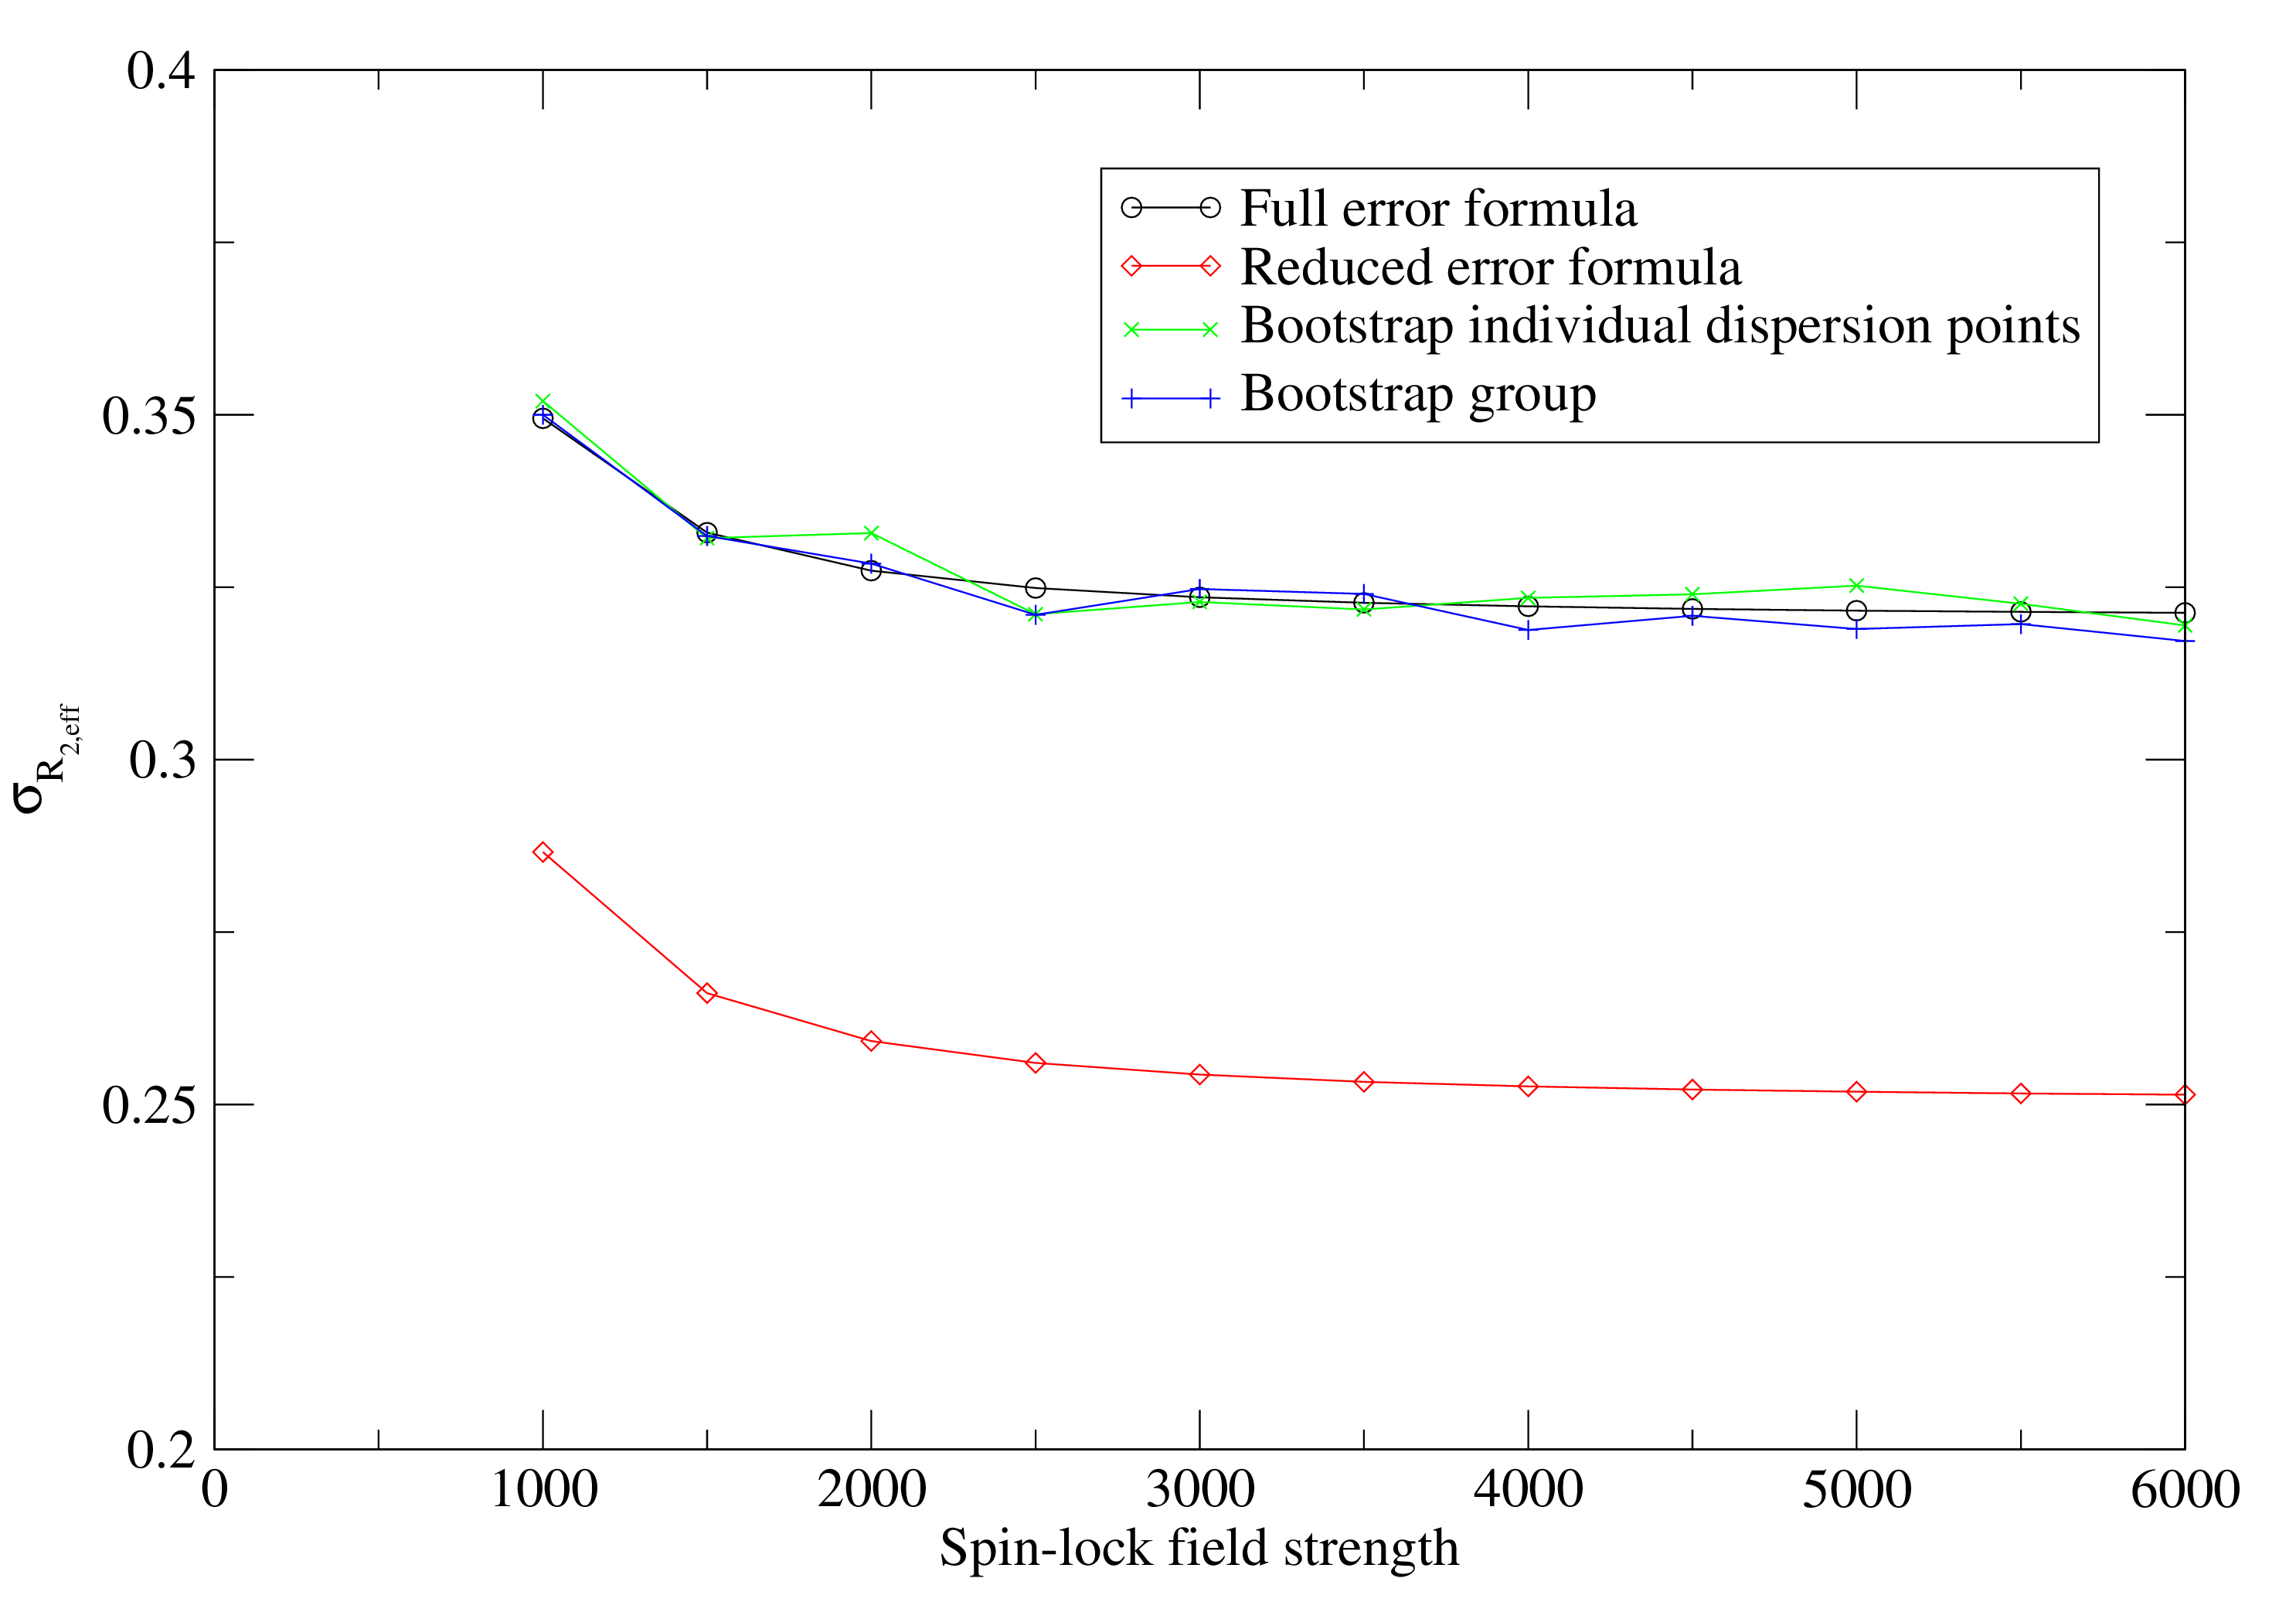
\includegraphics[width=0.9\textwidth, bb=14 14 728 512]{graphics/analyses/dispersion/error_comparison}}
\caption[Comparison of relaxation dispersion errors]{A demonstration of the inaccuracy of the error formula of Equation~\ref{eq: IT05 dispersion error} from \citet{IshimaTorchia05}.  This plot was generated using the script \file{test\_suite/shared\_data/dispersion/error\_testing/simulation.py}.  The bootstrapping simulation involves randomising noise-free $I_0$ and $I_1$ values for each dispersion data point assuming Gaussian errors.  The full error formula is from Equation~\ref{eq: dispersion error}, the reduced error formula is from Equation~\ref{eq: IT05 dispersion error}, the bootstrapping using individual dispersion points estimates the errors assuming different $I_0$ randomisations for each dispersion point and each simulation, and the bootstrapping group graph uses the same randomised $I_0$ value for all dispersion points for each simulation.}
\end{figure*}


% Variable relaxation period experiments.
\subsubsection{Variable relaxation period experiments}

For the variable relaxation time period type experiments, the $\Rtwoeff$/$\Ronerho$ values are determined by fitting to the simple two parameter exponential as in a $\Rone$ or $\Rtwo$ analysis.  Both $\Rtwoeff$/$\Ronerho$ and the initial peak intensity $I_0$ are optimised using the minimise user function for each exponential curve separately.  Monte Carlo simulations are used to obtain the parameter errors.



% No Rex model.
%~~~~~~~~~~~~~~

\subsection{The model for no chemical exchange relaxation}
\label{sect: dispersion: No Rex model}
\index{relaxation dispersion!No Rex model|textbf}

This model is provided for model selection purposes.  In combination with frequentist methods, such as AIC\index{model selection!AIC}, or Bayesian methods\index{model selection!Bayesian} it can show if the presence of chemical exchange is statistically significant.  Optimisation is still required as one $\Rtwozero$ value per magnetic field strength will be fit to the measured data for each spin system.  It is selected by setting the model to `No Rex'.



% The analytic CPMG models.
%%%%%%%%%%%%%%%%%%%%%%%%%%%

\section{The analytic CPMG models}
\label{sect: dispersion: analytic CPMG models}
\index{relaxation dispersion!Analytic CPMG model|textbf}

\begin{sidewaystable}
\begin{center}
\caption{The analytic and numerical models for CPMG-type experiments currently supported within relax}
\begin{tabular}{lllcll}
\toprule
Model code               & Solution & Sites & Parameters                                          & Restriction                       & Reference \\
\midrule                                    
R2eff                    & -        & -     & $\{\Rtwoeff, \cdots\}$                              & Fixed relaxation time period      & - \\
R2eff                    & -        & -     & $\{\Rtwoeff, I_0, \cdots\}$                         & Variable relaxation time period   & - \\
No Rex                   & Closed   & 0     & $\{\Rtwozero, \cdots\}$                             & -                                 & - \\
LM63                     & Analytic & 2     & $\{\Rtwozero, \dots, \Phiex, \kex\}$                & Fast exchange                     & \citet{LuzMeiboom63} \\
LM63 3-site              & Analytic & 3     & $\{\Rtwozero, \dots, \PhiexB, \kB, \PhiexC, \kC\}$  & Fast exchange, $\pA > \pB$ and $\pA > \pC$  & \citet{LuzMeiboom63} \\
CR72                     & Analytic & 2     & $\{\Rtwozero, \dots, \pA, \dw, \kex\}$              & $\pA > \pB$                       & \citet{CarverRichards72} \\
CR72 full                & Analytic & 2     & $\{\RtwozeroA, \RtwozeroB, \dots, \pA, \dw, \kex\}$ & $\pA > \pB$                       & \citet{CarverRichards72} \\
IT99                     & Analytic & 2     & $\{\Rtwozero, \dots, \Phiex, \pA.\dw^2, \kex\}$     & $\pA \gg \pB$                     & \citet{IshimaTorchia99} \\
TSMFK01                  & Analytic & 2     & $\{\RtwozeroA, \dots, \dw, \kAB\}$                  & $\pA \gg \pB$                     & \citet{Tollinger01} \\
NS CPMG 2-site 3D        & Numeric  & 2     & $\{\Rtwozero, \dots, \pA, \dw, \kex\}$              & $\pA > \pB$                       & - \\
NS CPMG 2-site 3D full   & Numeric  & 2     & $\{\RtwozeroA, \RtwozeroB, \dots, \pA, \dw, \kex\}$ & $\pA > \pB$                       & - \\
NS CPMG 2-site star      & Numeric  & 2     & $\{\Rtwozero, \dots, \pA, \dw, \kex\}$              & $\pA > \pB$                       & - \\
NS CPMG 2-site star full & Numeric  & 2     & $\{\RtwozeroA, \RtwozeroB, \dots, \pA, \dw, \kex\}$ & $\pA > \pB$                       & - \\
NS CPMG 2-site expanded  & Numeric  & 2     & $\{\Rtwozero, \dots, \pA, \dw, \kex\}$              & $\pA > \pB$                       & - \\
\bottomrule
\label{table: CPMG dispersion models}
\end{tabular}
\end{center}
\end{sidewaystable}



% LM63 model.
%~~~~~~~~~~~~

\subsection{The LM63 2-site fast exchange CPMG model}
\label{sect: dispersion: LM63 model}
\index{relaxation dispersion!LM63 model|textbf}

This is the original model for 2-site fast exchange for CPMG-type experiments.
It is selected by setting the model to `LM63', here named after \citet{LuzMeiboom63}.
The original $n$-site Equation~(7) from their paper can be written as:
\begin{equation}
    \Rex = \left[ 1 - 2\tex\taucpmg \cdot \tanh \left( 2\tex\taucpmg \right)^{-1} \right] \cdot \tex \cdot \sum_{i=2}^n p_\textrm{i}\dw_{i} ,
\end{equation}

or rearranged as:
\begin{equation} \label{eq: Luz-Meiboom}
    \Rex = \sum_{i=2}^n \frac{\Phi_\textrm{ex,i}}{\textrm{k}_\textrm{i}} \cdot \left( 1 - \frac{4\nucpmg}{\textrm{k}_\textrm{i}} \cdot \tanh \left( \frac{\textrm{k}_\textrm{i}}{4\nucpmg} \right) \right) ,
\end{equation}


The equation for the 2-site exchange process can be expressed as:
\begin{equation}
    \Rtwoeff = \Rtwozero + \frac{\Phiex}{\kex} \cdot \left( 1 - \frac{4\nucpmg}{\kex} \cdot \tanh \left( \frac{\kex}{4\nucpmg} \right) \right) .
\end{equation}

The reference for this equation is:
\begin{itemize}
\item \bibentry{LuzMeiboom63}
\end{itemize}


% LM63 3-site model.
%~~~~~~~~~~~~~~~~~~~

\subsection{The LM63 3-site fast exchange CPMG model}
\label{sect: dispersion: LM63 3-site model}
\index{relaxation dispersion!LM63 3-site model|textbf}

This is the original \citet{LuzMeiboom63} model for 3-site fast exchange for CPMG-type experiments.
It is selected by setting the model to `LM63 3-site'.
Taking the original Equation~\ref{eq: Luz-Meiboom}, the equation for 3-site exchange is simply:
\begin{equation}
    \Rex = \sum_{i=2}^3 \frac{\Phi_\textrm{ex,i}}{\textrm{k}_\textrm{i}} \cdot \left( 1 - \frac{4\nucpmg}{\textrm{k}_\textrm{i}} \cdot \tanh \left( \frac{\textrm{k}_\textrm{i}}{4\nucpmg} \right) \right) ,
\end{equation}

The reference for this equation is:
\begin{itemize}
\item \bibentry{LuzMeiboom63}
\end{itemize}

This model is only provided as a demonstration and should not be used for a normal analysis.
Without data at multiple temperatures, a feature not currently supported within relax, that there are infinite lines of solutions and that the $\PhiexB$, $\PhiexC$, $\kB$ and $\kC$ parameters are all convoluted together.

This equation was made more practically relevant in the paper of \citet{OConnell09}.
This relies on the assumption that site~1 (or~A) has a much larger equilibrium population than the other sites ($\pA \gg \pB$ and $\pA \gg \pC$).
As stated, ``if the different values of ji are well-separated (by a factor of 3-10), then Eq.~3 reduces approximately to the sum of n~-~1 independent two-state processes for exchange between site~1 and the n~-~1 other sites''.
In this situation, the following relationships hold
\begin{subequations}
\begin{align}
    &\kB \approx \kexB = \kAB + \kBA , \\
    &\kC \approx \kexC = \kAC + \kCA ,
\end{align}
\end{subequations}

and
\begin{subequations}
\begin{align}
    &\PhiexB = \overline{\Phiex} \frac{\kexB^2 \left( \overline{\kex} - \kexC \right)}{\kex^2 \left( \kex - \kexC \right)} , \label{eq: disp phiexB} \\
    &\PhiexC = \overline{\Phiex} \frac{\kexC^2 \left( \overline{\kex} - \kexB \right)}{\kex^2 \left( \kexC - \kexB \right)} , \label{eq: disp phiexC}
\end{align}
\end{subequations}

with
\begin{subequations}
\begin{align}
    &\overline{\PhiexB} \approx (\pA + \pC) \pB \dwAB^2 , \\
    &\overline{\PhiexC} \approx (\pA + \pB) \pC \dwAC^2 .
\end{align}
\end{subequations}

The parameter deconvolutions for this model can be performed after a relax analysis, if desired.



% Full CR72 model.
%~~~~~~~~~~~~~~~~~

\subsection{The full CR72 2-site CPMG model}
\label{sect: dispersion: CR72 full model}
\index{relaxation dispersion!CR72 full model|textbf}

This is the model for 2-site exchange on all times scales (with the constraint that $\pA > \pB$), named after \citet{CarverRichards72}.
It is selected by setting the model to `CR72 full'.
The equation is
\begin{equation}
    \Rtwoeff = \frac{1}{2} \Big( \textrm{R}_\textrm{2A}^0 + \textrm{R}_\textrm{2B}^0 + \kex - 2\nucpmg\cosh^{-1} \big( D_+\cosh(\eta_+) - D_-\cos(\eta_-) \big) \Big) ,
\end{equation}

where
\begin{align}
    D_\pm    &= \frac{1}{2} \left( \pm1 + \frac{\Psi + 2\dw^2}{\sqrt{\Psi^2 + \zeta^2}} \right) , \\
    \eta_\pm &= 2^{\frac{2}{3}}\frac{1}{\nucpmg} \left( \pm\Psi + \sqrt{\Psi^2 + \zeta^2} \right)^{\frac{1}{2}} , \\
    \Psi     &= \left( \textrm{R}_\textrm{2A}^0 - \textrm{R}_\textrm{2B}^0 - \pA\kex + \pB\kex \right)^2 - \dw^2 + 4\pA\pB\kex^2 , \\
    \zeta    &= 2\dw \left( \textrm{R}_\textrm{2A}^0 - \textrm{R}_\textrm{2B}^0 - \pA\kex + \pB\kex \right).
\end{align}

The reference for this equation is:
\begin{itemize}
\item \bibentry{CarverRichards72}
\end{itemize}



% CR72 model.
%~~~~~~~~~~~~

\subsection{The reduced CR72 2-site CPMG model}
\label{sect: dispersion: CR72 model}
\index{relaxation dispersion!CR72 model|textbf}

This is the model for 2-site exchange on all times scales (with the constraint that $\pA > \pB$), named after \citet{CarverRichards72}.
It is selected by setting the model to `CR72'.
It is the same as the full CR72 model described above, but with the simplification that $\RtwozeroA = \RtwozeroB$.
This simplifies the equations to
\begin{equation}
    \Rtwoeff = \Rtwozero + \frac{\kex}{2} - \nucpmg\cosh^{-1} \big( D_+\cosh(\eta_+) - D_-\cos(\eta_-) \big) ,
\end{equation}

where $D_\pm$ and $\eta_\pm$ are unchanged and
\begin{align}
    \Psi  &= \kex^2 - \dw^2 , \\
    \zeta &= -2\dw (\pA\kex - \pB\kex) .
\end{align}



% IT99 model.
%~~~~~~~~~~~~

\subsection{The IT99 2-site CPMG model}
\label{sect: dispersion: IT99 model}
\index{relaxation dispersion!IT99 model|textbf}

This is the model for 2-site exchange on all times scales (with the constraint that $\pA \gg \pB$), named after \citet{IshimaTorchia99}.  It is selected by setting the model to `IT99'.  The equation is:
\begin{align}
    \Rex       &\simeq \frac{\Phiex\tex}{1 + \omega_a^2\tex^2} , \\
    \omega_a^2 &= \sqrt{\omega_\textrm{1eff}^4 + \pA^2\dw^4} , \\
    \Rtwoeff   &= \Rtwozero + \Rex .
\end{align}

The effective rotating frame field for a CPMG-type experiment is given by
\begin{equation}
    \omega_\textrm{1eff} = 2\sqrt{3}\nucpmg ,
\end{equation}

and hence
\begin{equation}
    \omega_\textrm{1eff}^4 = 144\nucpmg^4 .
\end{equation}

The reference for this equation is:
\begin{itemize}
\item \bibentry{IshimaTorchia99}
\end{itemize}



% TSMFK01 model.
%~~~~~~~~~~~~

\subsection{The TSMFK01 2-site CPMG model}
\label{sect: dispersion: TSMFK01 model}
\index{relaxation dispersion!TSMFK01 model|textbf}



This is the model for 2-site very-slow exchange model for time scales within range of microsecond to second time scale, where $\pA \gg \pB$, and named after \citet{Tollinger01}.  It is selected by setting the model to `TSMFK01'.  A particularly interesting feature of the dispersion curves is the damped oscillations, which occur at low CPMG field strengths, and is solely a function of the chemical shift difference between the two sites (i.e., independent of the rate of exchange).  

The equation is:
\begin{align}
    \Rtwoeff = \RtwozeroA + \kAB - \kAB \frac{\sin{(\dw \cdot \taucpmg )}}{\dw \cdot \taucpmg}
\end{align}

The reference for this equation is:
\begin{itemize}
\item \bibentry{Tollinger01}
\end{itemize}



% The numeric CPMG models.
%%%%%%%%%%%%%%%%%%%%%%%%%%

\section{The numeric CPMG models}
\label{sect: dispersion: numeric CPMG models}
\index{relaxation dispersion!Numeric CPMG model|textbf}


% Full NS CPMG 2-site 3D model.
%~~~~~~~~~~~~~~~~~~~~~~~~~~~~~~

\subsection{The full NS 2-site 3D CPMG model}
\label{sect: dispersion: NS CPMG 2-site 3D full model}
\index{relaxation dispersion!NS CPMG 2-site 3D full model|textbf}

This is the numerical model for 2-site exchange using 3D magnetisation vectors.
It is selected by setting the model to `NS CPMG 2-site 3D full'.
The simple constraint $\pA > \pB$ is used to halve the optimisation space, as both sides of the limit are mirror image spaces.


% Reduced NS CPMG 2-site 3D model.
%~~~~~~~~~~~~~~~~~~~~~~~~~~~~~~~~~

\subsection{The reduced NS 2-site 3D CPMG model}
\label{sect: dispersion: NS CPMG 2-site 3D model}
\index{relaxation dispersion!NS CPMG 2-site 3D model|textbf}

This is the numerical model for 2-site exchange using 3D magnetisation vectors, whereby the simplification $\RtwozeroA = \RtwozeroB$ is assumed.
It is selected by setting the model to `NS CPMG 2-site 3D'.
The simple constraint $\pA > \pB$ is used to halve the optimisation space, as both sides of the limit are mirror image spaces.


% Full NS CPMG 2-site star model.
%~~~~~~~~~~~~~~~~~~~~~~~~~~~~~~~~

\subsection{The full NS 2-site star CPMG model}
\label{sect: dispersion: NS CPMG 2-site star full model}
\index{relaxation dispersion!NS CPMG 2-site star full model|textbf}

This is the numerical model for 2-site exchange using complex conjugate matrices.
It is selected by setting the model to `NS CPMG 2-site star full'.
The simple constraint $\pA > \pB$ is used to halve the optimisation space, as both sides of the limit are mirror image spaces.


% Reduced NS CPMG 2-site star model.
%~~~~~~~~~~~~~~~~~~~~~~~~~~~~~~~~~~~

\subsection{The reduced NS 2-site star CPMG model}
\label{sect: dispersion: NS CPMG 2-site star model}
\index{relaxation dispersion!NS CPMG 2-site star model|textbf}

This is the numerical model for 2-site exchange using complex conjugate matrices, whereby the simplification $\RtwozeroA = \RtwozeroB$ is assumed.
It is selected by setting the model to `NS CPMG 2-site star'.
The simple constraint $\pA > \pB$ is used to halve the optimisation space, as both sides of the limit are mirror image spaces.


% NS CPMG 2-site expanded model.
%~~~~~~~~~~~~~~~~~~~~~~~~~~~~~~~

\subsection{The NS 2-site expanded CPMG model}
\label{sect: dispersion: NS CPMG 2-site expanded model}
\index{relaxation dispersion!NS CPMG 2-site expanded model|textbf}

This is the numerical model for 2-site exchange expanded using Maple by Nikolai Skrynnikov.
It is selected by setting the model to `NS CPMG 2-site expanded'.
The simple constraint $\pA > \pB$ is used to halve the optimisation space, as both sides of the limit are mirror image spaces.



% The analytic R1rho models.
%%%%%%%%%%%%%%%%%%%%%%%%%%%

\section{The analytic $\Ronerho$ models}
\label{sect: dispersion: analytic R1rho models}
\index{relaxation dispersion!Analytic R1rho model|textbf}

\begin{sidewaystable}
\begin{center}
\caption{The analytic and numerical models for $\Ronerho$-type experiments currently supported within relax.}
\begin{tabular}{lllcll}
\toprule
Model code      & Solution & Sites & Parameters                                        & Restriction                       & Reference \\
\midrule                            
R2eff           & -        & -     & $\{\Ronerho, \cdots\}$                            & Fixed relaxation time period      & - \\
R2eff           & -        & -     & $\{\Ronerho, I_0, \cdots\}$                       & Variable relaxation time period   & - \\
No Rex          & Closed   & 0     & $\{\Ronerhoprime, \cdots\}$                       & -                                 & - \\
M61             & Analytic & 2     & $\{\Ronerhoprime, \dots, \Phiex, \kex\}$          & Fast exchange, on-resonance, $\Rone = \Rtwo$ & \citet{Meiboom61} \\
DPL94           & Analytic & 2     & $\{\Ronerhoprime, \dots, \Phiex, \kex\}$          & Fast exchange                     & \citet{Davis94} \\
M61 skew        & Analytic & 2     & $\{\Ronerhoprime, \dots, \pA, \dw, \kex\}$        & $\pA \gg \pB$, on-resonance       & \citet{Meiboom61} \\
TP02            & Analytic & 2     & $\{\Ronerhoprime, \dots, \pA, \dw, \kex\}$        & Not fast exchange                 & \citet{TrottPalmer02} \\
NS R1rho 2-site & Numeric  & 2     & $\{\Ronerhoprime, \dots, \pA, \dw, \kex\}$        & $\pA > \pB$                       & - \\
\bottomrule
\label{table: R1rho dispersion models}
\end{tabular}
\end{center}
\end{sidewaystable}


% M61 model.
%~~~~~~~~~~~

\subsection{The M61 2-site fast exchange $\Ronerho$ model}
\label{sect: dispersion: M61 model}
\index{relaxation dispersion!M61 model|textbf}

This is the model for 2-site fast exchange for on-resonance $\Ronerho$-type experiments.  It is selected by setting the model to `M61', here named after \citet{Meiboom61}.  The equation for the exchange process is:
\begin{equation}
    \Ronerho = \Ronerhoprime + \frac{\Phiex\kex}{\kex^2 + \omegae^2} .
\end{equation}

The reference for this equation is:
\begin{itemize}
\item \bibentry{Meiboom61}
\end{itemize}


% M61 skew model.
%~~~~~~~~~~~~~~~~

\subsection{The M61 skew 2-site fast exchange $\Ronerho$ model}
\label{sect: dispersion: M61 skew model}
\index{relaxation dispersion!M61 skew model|textbf}

This is the second model for 2-site fast exchange for on-resonance $\Ronerho$-type experiments from \citet{Meiboom61}.  It is selected by setting the model to `M61 skew'.  The equation for the exchange process is:
\begin{equation}
    \Ronerho = \Ronerhoprime + \frac{\pA^2\pB\dw^2\kex}{\kex^2 + \pA^2\dw^2 + \omegaone^2} .
\end{equation}

Care must be taken as this model appears to have infinite lines of solutions -- $\pA$ and $\dw$ are convoluted.  Hence this model is disabled in the dispersion auto-analysis.


% DPL94 model.
%~~~~~~~~~~~~~

\subsection{The DPL94 2-site fast exchange $\Ronerho$ model}
\label{sect: dispersion: DPL94 model}
\index{relaxation dispersion!DPL94 model|textbf}

This is the model for 2-site fast exchange for $\Ronerho$-type experiments.  It is selected by setting the model to `DPL94', here named after \citet{Davis94}.  It extends the \citet{Meiboom61} model to off-resonance data.  The model collapses to the M61 model for on-resonance data.  The equation for the exchange process is:
\begin{equation}
    \Ronerho = \Rone \cos^2\theta  +  \left( \Ronerhoprime + \frac{\Phiex\kex}{\kex^2 + \omegae^2} \right) \sin^2\theta ,
\end{equation}

where $\theta$ is the rotating frame tilt angle.  The reference for this equation is:
\begin{itemize}
\item \bibentry{Davis94}
\end{itemize}


% TP02 model.
%~~~~~~~~~~~~

\subsection{The TP02 2-site exchange $\Ronerho$ model}
\label{sect: dispersion: TP02 model}
\index{relaxation dispersion!TP02 model|textbf}

This is the model for 2-site exchange for off-resonance $\Ronerho$-type experiments from \citet{TrottPalmer02}.  It is selected by setting the model to `TP02'.  The equation for the exchange process is:
\begin{equation}
    \Ronerho = \Rone\cos^2\theta + \left( \Ronerhoprime + \frac{\pA\pB\dw^2\kex}{\omega_\textrm{Aeff}^2\omega_\textrm{Beff}^2/\omega_\textrm{eff}^2 + \kex^2} \right) \sin^2\theta.
\end{equation}



% The numeric R1rho models.
%%%%%%%%%%%%%%%%%%%%%%%%%%%

\section{The numeric $\Ronerho$ models}
\label{sect: dispersion: numeric R1rho models}
\index{relaxation dispersion!Numeric R1rho model|textbf}

% NS R1rho 2-site model.
%~~~~~~~~~~~~~~~~~~~~~~~

\subsection{The NS 2-site $\Ronerho$ model}
\label{sect: dispersion: NS R1rho 2-site model}
\index{relaxation dispersion!NS R1rho 2-site model|textbf}

This is the numerical model for 2-site exchange using 3D magnetisation vectors.
It is selected by setting the model to `NS R1rho 2-site'.
The simple constraint $\pA > \pB$ is used to halve the optimisation space, as both sides of the limit are mirror image spaces.



% Script UI.
%%%%%%%%%%%%

\section{Analysing dispersion in the prompt/script UI mode}

Before reading this section, please read Chapter~\ref{ch: data model} covering the relax data model first.  It will explain many of the concepts used within the following example script.


% The sample script.
%~~~~~~~~~~~~~~~~~~~

\subsection{Dispersion script mode -- the sample script}

The following is a verbatim copy of the contents of the \file{sample\_scripts/relax\_disp/\linebreak[0]{}cpmg\_analysis.py} file.
You will need to first copy this script to a dedicated analysis directory containing peak lists, a sequence or PDB file and a file listing unresolved spin systems, and then modify its contents to suit your specific analysis.
The script contents are:

\begin{lstlisting}
"""Script for performing a full relaxation dispersion analysis using CPMG-type data."""


# Python module imports.
from os import sep

# relax module imports.
from auto_analyses.relax_disp import Relax_disp


# Analysis variables.
#####################

# The dispersion models.
MODELS = ['R2eff', 'No Rex', 'LM63', 'CR72', 'IT99', 'TSMFK01', 'NS CPMG 2-site expanded']

# The grid search size (the number of increments per dimension).
GRID_INC = 21

# The number of Monte Carlo simulations to be used for error analysis at the end of the analysis.
MC_NUM = 500

# The model selection technique to use.
MODSEL = 'AIC'


# Set up the data pipe.
#######################

# Create the data pipe.
pipe_name = 'base pipe'
pipe_bundle = 'relax_disp'
pipe.create(pipe_name=pipe_name, bundle=pipe_bundle, pipe_type='relax_disp')

# Load the sequence.
sequence.read('fake_sequence.in', res_num_col=1, res_name_col=2)

# Name the spins so they can be matched to the assignments, and the isotope for field strength scaling.
spin.name(name='N')
spin.isotope(isotope='15N')

# The spectral data - spectrum ID, peak list file name, CPMG frequency (Hz), spectrometer frequency in Hertz.
data = [
    ['500_reference.in',    '500_MHz'+sep+'reference.in_sparky',           None,  500e6],
    ['500_66.667.in',       '500_MHz'+sep+'66.667.in_sparky',           66.6666,  500e6],
    ['500_133.33.in',       '500_MHz'+sep+'133.33.in_sparky',          133.3333,  500e6],
    ['500_133.33.in.bis',   '500_MHz'+sep+'133.33.in.bis_sparky',      133.3333,  500e6],
    ['500_200.in',          '500_MHz'+sep+'200.in_sparky',             200.0000,  500e6],
    ['500_266.67.in',       '500_MHz'+sep+'266.67.in_sparky',          266.6666,  500e6],
    ['500_333.33.in',       '500_MHz'+sep+'333.33.in_sparky',          333.3333,  500e6],
    ['500_400.in',          '500_MHz'+sep+'400.in_sparky',             400.0000,  500e6],
    ['500_466.67.in',       '500_MHz'+sep+'466.67.in_sparky',          466.6666,  500e6],
    ['500_533.33.in',       '500_MHz'+sep+'533.33.in_sparky',          533.3333,  500e6],
    ['500_533.33.in.bis',   '500_MHz'+sep+'533.33.in.bis_sparky',      533.3333,  500e6],
    ['500_600.in',          '500_MHz'+sep+'600.in_sparky',             600.0000,  500e6],
    ['500_666.67.in',       '500_MHz'+sep+'666.67.in_sparky',          666.6666,  500e6],
    ['500_733.33.in',       '500_MHz'+sep+'733.33.in_sparky',          733.3333,  500e6],
    ['500_800.in',          '500_MHz'+sep+'800.in_sparky',             800.0000,  500e6],
    ['500_866.67.in',       '500_MHz'+sep+'866.67.in_sparky',          866.6666,  500e6],
    ['500_933.33.in',       '500_MHz'+sep+'933.33.in_sparky',          933.3333,  500e6],
    ['500_933.33.in.bis',   '500_MHz'+sep+'933.33.in.bis_sparky',      933.3333,  500e6],
    ['500_1000.in',         '500_MHz'+sep+'1000.in_sparky',           1000.0000,  500e6],
    ['800_reference.in',    '800_MHz'+sep+'reference.in_sparky',           None,  800e6],
    ['800_66.667.in',       '800_MHz'+sep+'66.667.in_sparky',           66.6666,  800e6],
    ['800_133.33.in',       '800_MHz'+sep+'133.33.in_sparky',          133.3333,  800e6],
    ['800_133.33.in.bis',   '800_MHz'+sep+'133.33.in.bis_sparky',      133.3333,  800e6],
    ['800_200.in',          '800_MHz'+sep+'200.in_sparky',             200.0000,  800e6],
    ['800_266.67.in',       '800_MHz'+sep+'266.67.in_sparky',          266.6666,  800e6],
    ['800_333.33.in',       '800_MHz'+sep+'333.33.in_sparky',          333.3333,  800e6],
    ['800_400.in',          '800_MHz'+sep+'400.in_sparky',             400.0000,  800e6],
    ['800_466.67.in',       '800_MHz'+sep+'466.67.in_sparky',          466.6666,  800e6],
    ['800_533.33.in',       '800_MHz'+sep+'533.33.in_sparky',          533.3333,  800e6],
    ['800_533.33.in.bis',   '800_MHz'+sep+'533.33.in.bis_sparky',      533.3333,  800e6],
    ['800_600.in',          '800_MHz'+sep+'600.in_sparky',             600.0000,  800e6],
    ['800_666.67.in',       '800_MHz'+sep+'666.67.in_sparky',          666.6666,  800e6],
    ['800_733.33.in',       '800_MHz'+sep+'733.33.in_sparky',          733.3333,  800e6],
    ['800_800.in',          '800_MHz'+sep+'800.in_sparky',             800.0000,  800e6],
    ['800_866.67.in',       '800_MHz'+sep+'866.67.in_sparky',          866.6666,  800e6],
    ['800_933.33.in',       '800_MHz'+sep+'933.33.in_sparky',          933.3333,  800e6],
    ['800_933.33.in.bis',   '800_MHz'+sep+'933.33.in.bis_sparky',      933.3333,  800e6],
    ['800_1000.in',         '800_MHz'+sep+'1000.in_sparky',           1000.0000,  800e6]
]

# Loop over the spectra.
for id, file, cpmg_frq, H_frq in data:
    # Load the peak intensities.
    spectrum.read_intensities(file=file, spectrum_id=id, int_method='height')

    # Set the relaxation dispersion experiment type.
    relax_disp.exp_type(spectrum_id=id, exp_type='CPMG')

    # Set the relaxation dispersion CPMG frequencies.
    relax_disp.cpmg_frq(spectrum_id=id, cpmg_frq=cpmg_frq)

    # Set the NMR field strength of the spectrum.
    spectrometer.frequency(id=id, frq=H_frq)

    # Relaxation dispersion CPMG constant time delay T (in s).
    relax_disp.relax_time(spectrum_id=id, time=0.030)

# Specify the duplicated spectra.
spectrum.replicated(spectrum_ids=['500_133.33.in', '500_133.33.in.bis'])
spectrum.replicated(spectrum_ids=['500_533.33.in', '500_533.33.in.bis'])
spectrum.replicated(spectrum_ids=['500_933.33.in', '500_933.33.in.bis'])
spectrum.replicated(spectrum_ids=['800_133.33.in', '800_133.33.in.bis'])
spectrum.replicated(spectrum_ids=['800_533.33.in', '800_533.33.in.bis'])
spectrum.replicated(spectrum_ids=['800_933.33.in', '800_933.33.in.bis'])

# Peak intensity error analysis.
spectrum.error_analysis(subset=['500_reference.in', '500_66.667.in', '500_133.33.in', '500_133.33.in.bis', '500_200.in', '500_266.67.in', '500_333.33.in', '500_400.in', '500_466.67.in', '500_533.33.in', '500_533.33.in.bis', '500_600.in', '500_666.67.in', '500_733.33.in', '500_800.in', '500_866.67.in', '500_933.33.in', '500_933.33.in.bis', '500_1000.in'])
spectrum.error_analysis(subset=['800_reference.in', '800_66.667.in', '800_133.33.in', '800_133.33.in.bis', '800_200.in', '800_266.67.in', '800_333.33.in', '800_400.in', '800_466.67.in', '800_533.33.in', '800_533.33.in.bis', '800_600.in', '800_666.67.in', '800_733.33.in', '800_800.in', '800_866.67.in', '800_933.33.in', '800_933.33.in.bis', '800_1000.in'])

# Deselect unresolved spins.
deselect.read(file='unresolved', dir='500_MHz', res_num_col=1)
deselect.read(file='unresolved', dir='800_MHz', res_num_col=1)



# Auto-analysis execution.
##########################

# Do not change!
Relax_disp(pipe_name=pipe_name, pipe_bundle=pipe_bundle, models=MODELS, grid_inc=GRID_INC, mc_sim_num=MC_NUM, modsel=MODSEL)
\end{lstlisting}


% The imports.
%~~~~~~~~~~~~~

\subsection{Dispersion script mode -- imports} \label{sect: dispersion script imports}

At the very start of the script are two import statements.  This is simply the standard Python import system for modules.  The first will import the \pycode{sep} variable which is the operating system independent directory separator:

\begin{lstlisting}[firstnumber=4]
# Python module imports.
from os import sep
\end{lstlisting}

This \pycode{sep} variable will be used later on in the script.  The second import is that of the automated relaxation dispersion class \pycode{Relax\_disp} which will be used at the very end of the script to perform the full analysis:

\begin{lstlisting}[firstnumber=7]
# relax module imports.
from auto_analyses.relax_disp import Relax_disp
\end{lstlisting}


% The analysis variables.
%~~~~~~~~~~~~~~~~~~~~~~~~

\subsection{Dispersion script mode -- analysis variables} \label{sect: dispersion script variables}

The next part of the script is the definition of a number of analysis variables.  As the example in this section is for CPMG-type experiments, the relaxation dispersion models which will be used in the auto-analysis are:

\begin{lstlisting}[firstnumber=14]
# The dispersion models.
MODELS = ['R2eff', 'No Rex', 'LM63', 'CR72', 'IT99', 'TSMFK01', 'NS CPMG 2-site expanded']
\end{lstlisting}

If you have $\Ronerho$-type data, the models could be changed to:

\begin{lstlisting}[numbers=none]
# The dispersion models.
MODELS = ['R2eff', 'No Rex', 'M61', 'DPL72', 'TP02']
\end{lstlisting}

The next variable affects the optimisation precision:

\begin{lstlisting}[firstnumber=17]
# The grid search size (the number of increments per dimension).
GRID_INC = 21
\end{lstlisting}

The number of grid search increments may be decreased, but only after careful checking with a higher number of increments.  Setting this value too low may place the initial optimisation too far away from the minimum.  Although as-of-yet undetected and unpublished, if multiple local minima do exist then optimisation may not reach the global minimum.  Too little grid search increments can also cause the total optimisation time to increase as the Nelder-Mead simplex\index{optimisation!simplex algorithm}\index{optimisation!Nelder-Mead algorithm} optimisation together with the Logarithmic-barrier penalty function\index{optimisation!logarithmic-barrier penalty function} as used in the auto-analysis may require more time to reach the minimum.

The Monte Carlo simulation\index{Monte Carlo simulation} number \pycode{MC\_NUM} variable affects the error estimate precision:

\begin{lstlisting}[firstnumber=20]
# The number of Monte Carlo simulations to be used for error analysis at the end of the analysis.
MC_NUM = 500
\end{lstlisting}

For accurate parameter errors this number should not be decreased.  Ideally it should be increased however this will significantly increase the total analysis time.

The last variable defines how the best dispersion model for the measured data is chosen:

\begin{lstlisting}[firstnumber=23]
# The model selection technique to use.
MODSEL = 'AIC'
\end{lstlisting}

For the automated analysis, currently only AIC\index{model selection!AIC}, AICc\index{model selection!AICc}, and BIC\index{model selection!BIC} are supported.  For details about these frequentist\index{model selection!frequentist} model selection techniques and their application to NMR data, see \citet{dAuvergneGooley03}.  Post-analysis comparisons can also be preformed if desired.


% Initialisation of the data pipe.
%~~~~~~~~~~~~~~~~~~~~~~~~~~~~~~~~~

\subsection{Dispersion script mode -- initialisation of the data pipe} \label{sect: dispersion initialisation}

The data pipe is created using the lines:

\begin{lstlisting}[firstnumber=30]
# Create the data pipe.
pipe_name = 'base pipe'
pipe_bundle = 'relax_disp'
pipe.create(pipe_name=pipe_name, bundle=pipe_bundle, pipe_type='relax_disp')
\end{lstlisting}

The first two lines define variables for the data pipe name and the pipe bundle name.  The pipe bundle is used to group together all of the data pipes created by the automated protocol.  See section~\ref{sect: data pipe bundles} on page~\pageref{sect: data pipe bundles} for more details.

The \uf{pipe.create} user function will then create a relaxation dispersion specific data pipe labelled with the pipe and bundle names.  The third argument sets the pipe type to that of relaxation dispersion.  The rest of the script is used to fill this base data pipe with all of the data required for a dispersion analysis.  The auto-analysis will then copy the data from this pipe as it sees fit.


% Spin systems.
%~~~~~~~~~~~~~~

\subsection{Dispersion script mode -- setting up the spin systems}

The first thing which needs to be completed prior to any spin specific command is to generate the molecule, residue and spin data structures for storing the spin specific data.  In the sample script above, this is generated from a plain text file with the sequence information, however a PDB file can be used instead (see the \uf{structure.read\_pdb} user function on page~\pageref{uf: structure.read_pdb} for more details).  In the case of the sample script, the command:

\begin{lstlisting}[firstnumber=35]
# Load the sequence.
sequence.read('fake_sequence.in', res_num_col=1, res_name_col=2)
\end{lstlisting}

will load residue names and numbers from the \file{fake\_sequence.in} file into relax, creating one spin per residue.  Then:

\begin{lstlisting}[firstnumber=38]
# Name the spins so they can be matched to the assignments, and the isotope for field strength scaling.
spin.name(name='N')
spin.isotope(isotope='15N')
\end{lstlisting}

will set up the spin information required for loading the peak intensity data from Sparky peak lists and for the analysis of the dispersion data.


% Loading the data.
%~~~~~~~~~~~~~~~~~~

\subsection{Dispersion script mode -- loading the data}

To load the peak intensities\index{peak!intensity} into relax, a large data structure is first defined:

\begin{lstlisting}[firstnumber=42]
# The spectral data - spectrum ID, peak list file name, CPMG frequency (Hz), spectrometer frequency in Hertz.
data = [
    ['500_reference.in',    '500_MHz'+sep+'reference.in_sparky',           None,  500e6],
    ['500_66.667.in',       '500_MHz'+sep+'66.667.in_sparky',           66.6666,  500e6],
    ['500_133.33.in',       '500_MHz'+sep+'133.33.in_sparky',          133.3333,  500e6],
    ['500_133.33.in.bis',   '500_MHz'+sep+'133.33.in.bis_sparky',      133.3333,  500e6],
    ['500_200.in',          '500_MHz'+sep+'200.in_sparky',             200.0000,  500e6],
    ['500_266.67.in',       '500_MHz'+sep+'266.67.in_sparky',          266.6666,  500e6],
    ['500_333.33.in',       '500_MHz'+sep+'333.33.in_sparky',          333.3333,  500e6],
    ['500_400.in',          '500_MHz'+sep+'400.in_sparky',             400.0000,  500e6],
    ['500_466.67.in',       '500_MHz'+sep+'466.67.in_sparky',          466.6666,  500e6],
    ['500_533.33.in',       '500_MHz'+sep+'533.33.in_sparky',          533.3333,  500e6],
    ['500_533.33.in.bis',   '500_MHz'+sep+'533.33.in.bis_sparky',      533.3333,  500e6],
    ['500_600.in',          '500_MHz'+sep+'600.in_sparky',             600.0000,  500e6],
    ['500_666.67.in',       '500_MHz'+sep+'666.67.in_sparky',          666.6666,  500e6],
    ['500_733.33.in',       '500_MHz'+sep+'733.33.in_sparky',          733.3333,  500e6],
    ['500_800.in',          '500_MHz'+sep+'800.in_sparky',             800.0000,  500e6],
    ['500_866.67.in',       '500_MHz'+sep+'866.67.in_sparky',          866.6666,  500e6],
    ['500_933.33.in',       '500_MHz'+sep+'933.33.in_sparky',          933.3333,  500e6],
    ['500_933.33.in.bis',   '500_MHz'+sep+'933.33.in.bis_sparky',      933.3333,  500e6],
    ['500_1000.in',         '500_MHz'+sep+'1000.in_sparky',           1000.0000,  500e6],
    ['800_reference.in',    '800_MHz'+sep+'reference.in_sparky',           None,  800e6],
    ['800_66.667.in',       '800_MHz'+sep+'66.667.in_sparky',           66.6666,  800e6],
    ['800_133.33.in',       '800_MHz'+sep+'133.33.in_sparky',          133.3333,  800e6],
    ['800_133.33.in.bis',   '800_MHz'+sep+'133.33.in.bis_sparky',      133.3333,  800e6],
    ['800_200.in',          '800_MHz'+sep+'200.in_sparky',             200.0000,  800e6],
    ['800_266.67.in',       '800_MHz'+sep+'266.67.in_sparky',          266.6666,  800e6],
    ['800_333.33.in',       '800_MHz'+sep+'333.33.in_sparky',          333.3333,  800e6],
    ['800_400.in',          '800_MHz'+sep+'400.in_sparky',             400.0000,  800e6],
    ['800_466.67.in',       '800_MHz'+sep+'466.67.in_sparky',          466.6666,  800e6],
    ['800_533.33.in',       '800_MHz'+sep+'533.33.in_sparky',          533.3333,  800e6],
    ['800_533.33.in.bis',   '800_MHz'+sep+'533.33.in.bis_sparky',      533.3333,  800e6],
    ['800_600.in',          '800_MHz'+sep+'600.in_sparky',             600.0000,  800e6],
    ['800_666.67.in',       '800_MHz'+sep+'666.67.in_sparky',          666.6666,  800e6],
    ['800_733.33.in',       '800_MHz'+sep+'733.33.in_sparky',          733.3333,  800e6],
    ['800_800.in',          '800_MHz'+sep+'800.in_sparky',             800.0000,  800e6],
    ['800_866.67.in',       '800_MHz'+sep+'866.67.in_sparky',          866.6666,  800e6],
    ['800_933.33.in',       '800_MHz'+sep+'933.33.in_sparky',          933.3333,  800e6],
    ['800_933.33.in.bis',   '800_MHz'+sep+'933.33.in.bis_sparky',      933.3333,  800e6],
    ['800_1000.in',         '800_MHz'+sep+'1000.in_sparky',           1000.0000,  800e6]
]
\end{lstlisting}

In Python terminology, this is a list of lists data structure.  It is essentially a matrix of information which is used in the subsequent \pycode{for} loop.  The comment explains what each element is.  For $\Ronerho$-type experiments, the CPMG frequency column can be replaced with the spin-lock field strength.  This data structure will need to be tailored to your data.  It can be seen that the \pycode{sep} variable is now being used to specify that the Sparky files are either located in the \directory{500\_MHz} or \directory{800\_MHz} directories.  It is used here to make this script independent of the operating system.

The Python \pycode{for} loop starts with the lines:

\begin{lstlisting}[firstnumber=84]
# Loop over the spectra.
for id, file, cpmg_frq, H_frq in data:
\end{lstlisting}

and includes all subsequently indented lines.  This line of code takes the elements of the \pycode{data} data structure and splits it into 4 variables.  Therefore for the first line, \pycode{id} will be set to \pycode{`500\_reference.in'}, \pycode{file} will be set to \pycode{`500\_MHz/reference.in\_sparky'} on a Linux machine, \pycode{cpmg\_frq} will be \pycode{None}, and \pycode{H\_frq} will be 500~MHz.  For $\Ronerho$-type data, you could change the \pycode{cpmg\_frq} variable to \pycode{field} for example.

The first user function in the block loads the peak intensity data from the peak lists:

\begin{lstlisting}[firstnumber=86]
    # Load the peak intensities.
    spectrum.read_intensities(file=file, spectrum_id=id, int_method='height')
\end{lstlisting}

This assumes that peak heights were measured.  All data will be tagged with the given ID string.  For examples of peak list formats supported by relax, see Section~\ref{sect: Rx data loading} on page~\pageref{sect: Rx data loading}.
The next step is to specify the dispersion experiment type for each spectrum:

\begin{lstlisting}[firstnumber=89]
    # Set the relaxation dispersion experiment type.
    relax_disp.exp_type(spectrum_id=id, exp_type='CPMG')
\end{lstlisting}

This can either be \pycode{`CPMG'} or \pycode{`R1rho'}.
The next user function sets the CPMG frequencies for each spectrum:

\begin{lstlisting}[firstnumber=92]
    # Set the relaxation dispersion CPMG frequencies.
    relax_disp.cpmg_frq(spectrum_id=id, cpmg_frq=cpmg_frq)
\end{lstlisting}

For an $\Ronerho$-type experiment, these lines could be changed to:

\begin{lstlisting}[numbers=none]
    # Set the relaxation dispersion R1rho spin lock field strength.
    relax_disp.spin_lock_field(spectrum_id=id, field=field)
\end{lstlisting}

Then the NMR spectrometer field strength is set:

\begin{lstlisting}[firstnumber=95]
    # Set the NMR field strength of the spectrum.
    spectrometer.frequency(id=id, frq=H_frq)
\end{lstlisting}

And finally the relaxation time period is set with:

\begin{lstlisting}[firstnumber=98]
    # Relaxation dispersion CPMG constant time delay T (in s).
    relax_disp.relax_time(spectrum_id=id, time=0.030)
\end{lstlisting}

If exponential data has been collected rather than fixed time period data, then the \pycode{data} data structure can have an additional column added for the relaxation times, and then this same user function can be used.  The \pycode{for} loop will need one extra variable for the times, and this should be passed into this \uf{relax\_disp.relax\_time} user function for the time argument.

Finally, once the \pycode{for} loop has completed, replicated spectra are defined with the commands:

\begin{lstlisting}[firstnumber=101]
# Specify the duplicated spectra.
spectrum.replicated(spectrum_ids=['500_133.33.in', '500_133.33.in.bis'])
spectrum.replicated(spectrum_ids=['500_533.33.in', '500_533.33.in.bis'])
spectrum.replicated(spectrum_ids=['500_933.33.in', '500_933.33.in.bis'])
spectrum.replicated(spectrum_ids=['800_133.33.in', '800_133.33.in.bis'])
spectrum.replicated(spectrum_ids=['800_533.33.in', '800_533.33.in.bis'])
spectrum.replicated(spectrum_ids=['800_933.33.in', '800_933.33.in.bis'])
\end{lstlisting}


% The rest of the setup.
%~~~~~~~~~~~~~~~~~~~~~~~

\subsection{Dispersion script mode -- the rest of the setup} \label{sect: dispersion setup fin}

Once all the peak intensity data has been loaded a few calculations are required prior to optimisation.  Firstly the peak intensities for individual spins needs to be averaged across replicated spectra.  The peak intensity errors also have to be calculated using the standard deviation formula.  These two operations are executed by the user functions:

\begin{lstlisting}[firstnumber=109]
# Peak intensity error analysis.
spectrum.error_analysis(subset=['500_reference.in', '500_66.667.in', '500_133.33.in', '500_133.33.in.bis', '500_200.in', '500_266.67.in', '500_333.33.in', '500_400.in', '500_466.67.in', '500_533.33.in', '500_533.33.in.bis', '500_600.in', '500_666.67.in', '500_733.33.in', '500_800.in', '500_866.67.in', '500_933.33.in', '500_933.33.in.bis', '500_1000.in'])
spectrum.error_analysis(subset=['800_reference.in', '800_66.667.in', '800_133.33.in', '800_133.33.in.bis', '800_200.in', '800_266.67.in', '800_333.33.in', '800_400.in', '800_466.67.in', '800_533.33.in', '800_533.33.in.bis', '800_600.in', '800_666.67.in', '800_733.33.in', '800_800.in', '800_866.67.in', '800_933.33.in', '800_933.33.in.bis', '800_1000.in'])
\end{lstlisting}

Here the 500~MHz and 800~MHz peak intensity errors have been calculated separately as they should not be the same.

Any spins which cannot be resolved due to peak overlap were included in a file called \file{unresolved}.  This file can consist of optional columns of the molecule name, the residue name and number, and the spin name and number.  The matching spins are excluded from the analysis by the user functions:

\begin{lstlisting}[firstnumber=113]
# Deselect unresolved spins.
deselect.read(file='unresolved', dir='500_MHz', res_num_col=1)
deselect.read(file='unresolved', dir='800_MHz', res_num_col=1)
\end{lstlisting}


% Execution.
%~~~~~~~~~~~
\subsection{Dispersion script mode -- execution}

Once the data has set up and you have modified your script to match your analysis needs, then the data pipe, pipe bundle and analysis variables are passed into the \module{Relax\linebreak[0]{}\_disp} class.  This is the final lines of the script:

\begin{lstlisting}[firstnumber=119]
# Auto-analysis execution.
##########################

# Do not change!
Relax_disp(pipe_name=pipe_name, pipe_bundle=pipe_bundle, models=MODELS, grid_inc=GRID_INC, mc_sim_num=MC_NUM, modsel=MODSEL)
\end{lstlisting}

This will start the auto-analysis.



% Tutorial - adding models.
%%%%%%%%%%%%%%%%%%%%%%%%%%%

\section{Tutorial for adding relaxation dispersion models}
\label{sect: dispersion: model tutorial}

As the field of NMR relaxation dispersion has a very long history, it is not possible to include all analytic and numeric relaxation dispersion models for both CPMG-type\index{relaxation dispersion!CPMG-type experiment} or $\Ronerho$-type\index{relaxation dispersion!$\Ronerho$-type experiment} experiments in relax.  However it is not too difficult to add new models for your own needs if you have some Python, Matlab, Mathematica, or similar scripting skills.  The steps required are detailed on the \href{http://wiki.nmr-relax.com/}{relax wiki} page for the \href{http://wiki.nmr-relax.com/Tutorial\_for\_adding\_relaxation\_dispersion\_models\_to\_relax}{tutorial for adding relaxation dispersion models to relax}.
